%% [ADS 4-2005] Template file for 40in x 30in landscape poster
%%
%%
%%
%%
%% [ADS 4-2005] what follows here is obsolete I believe.
%%-------------------------------------------------------------------------
%% Written by Graeme, 2001-03 based on Norman's original microlensing
%% poster.
%%
%% $Id: poster-template-landscape.tex,v 1.1 2001/07/02 17:23:32 norman Exp $
%%
%% Default mode is landscape, which is what we want, however dvips and
%% a0poster do not quite do the right thing, so we end up with text in
%% landscape style (wide and short) down a portrait page (narrow and
%% long). Printing this onto the a0 printer chops the right hand edge.
%% However, 'psnup' can save the day, reorienting the text so that the
%% poster prints lengthways down an a0 portrait bounding box.
%%
%% 'psnup -w85cm -h119cm -f poster_from_dvips.ps poster_in_landscape.ps'
%%
%%-------------------------------------------------------------------------
%% Modified by Ronald Kumon, 06-2002 to incorporate a framebox border,
%%   add acknowledgments line at bottom, and change locations of logos
%%
%% Modified by Anand D. Sarwate 04-2005 to specialize to the UC Berkeley 
%%   EECS Wireless Foundaions conference poster template and for different
%%   paper sizes


%% [ADS 4-2005] latex --> dvips --> ps2pdf works just fine for me.
%%
%% To preview using xdvi:
%% 
%% $ xdvi -paper 1188x840mm -s 24 -nopostscript poster.dvi
%%
%% To convert dvi to Postscript:
%%
%% $ dvips -Ppdf -G0 -o poster.ps poster.dvi
%%
%% The dvips options are:
%% Ppdf: use the PDF printer configuration file
%% G0  : shift lower characters to higher position 
%%       (splits ligatures when using Times-Roman font)
%%
%% To convert Postscript to PDF:
%%
%% $ pstill -c -giptCQ -w 3368 -h 2378 -o poster.pdf poster.ps
%% ($ pstill -c -iptCQ -w 3225 -h 2378 -o poster.pdf poster.ps)
%%
%% Note that the pstill options are
%% c:  compression (more c's give more compression; up to four)
%% g:  take size from Postscript file
%% p:  include all fonts as partial fonts
%% i:  include all non-standard fonts
%% t:  map graphics transfer functions from PostScript to PDF. 
%% C:  use RGB color map
%% w:  width in points (1/72 inch) for 1188 mm
%% h:  height in points (1/72 inch) for 839 mm
%% Q:  take embedded fonts from PSFonts directory, not Postscript file
%% Note also that the -w and -h options need to be included else
%% some of the Postscript figures may not be displayed (particularly
%% those converted using fig2dev), even if the -g option is specified.
%% Also, the newest version of pstill (1.55.91) does not deal well with 
%% slanted Times Roman font; use italics or the older version (1.55.3). 
%%-------------------------------------------------------------------------


\documentclass{article}
%% [ADS 4/2005]  The template here does NOT make use of the 'slides'
%% option of Kumon in the interest of creating a more readable document
%% -- suggestions for how to make a backup style on separate sheet is
%% given in the text.
%%

%% If you want to number equations, set the equation number counter to zero.
%\setcounter{secnumdepth}{0}









%%%%%%%%%%%%%%%%%%%%%%%%%
%%% PACKAGE INCLUSION %%%
%%%%%%%%%%%%%%%%%%%%%%%%%

%% AMS packages for special symbols, etc
\usepackage{amsmath,amssymb}

\usepackage[round]{natbib}
\bibliographystyle{plainnat}

%\textsubscript
\usepackage{fixltx2e}
\usepackage{hyperref}

\usepackage{multirow}

\usepackage{soul}

\usepackage{qtree}  %syntax tree
%% This package gives you coloured text and various other simple
%% graphics hacks.  For details, see documentation in 
%% in /usr/local/teTeX/texmf/doc/generic/pstricks/*
\usepackage{pstricks}
\newrgbcolor{darkblue}{0.1 0.1 0.5}

%% The textpos package is necessary to position textblocks at arbitary 
%% places on the page.  Use showboxes option to show outlines of textboxes.
\usepackage[absolute]{textpos}
%\usepackage[absolute,showboxes]{textpos}

%% Package to include graphics.  
\usepackage{graphicx}
%% Define path for figures -- for safety, keep the last /
\graphicspath{{/your/figure/directory/here/if/any/}
{/an/second/directory/path/can/go/here/}}

%% Wrap text around figures
%\usepackage{wrapfig}

%% Use Times font instead of Computer Modern -- this gives better
%% appearance when resizing to large sixes.
%% Note that without the ``G0'' in the dvips conversion, 
%% all character combinations that will normally result in 
%% ligatures will have to be hacked to display properly.  For example, 
%%     fi --> \mbox{f}\mbox{i}
%% Other characters may also fail.  In addition, the Mathtimes font 
%% set should really be used for mathematics, but unfortunately they 
%% are only proprietary.  (The Computer Modern fonts may still look OK.)
\usepackage{times}

%% These colors are tried and tested for titles and headers. Don't
%% over use color!
%\usepackage[usenames]{color} % commented by Karol Kozioł
\usepackage{xcolor}
\definecolor{DarkBlue}{rgb}{0.1,0.1,0.5}
\definecolor{Black}{rgb}{0.0,0.0,0.0}
\definecolor{Red}{rgb}{0.6,0.0,0.2}
\definecolor{DarkBlue2}{rgb}{0.00,0.08,0.6}
\definecolor{DarkRed2}{rgb}{0.6,0.00,0.08}
\definecolor{DarkGreen2}{rgb}{0.00,0.6,0.08}

%% Load shadow box package
%\usepackage{shadow}

%% This loads font sizes in style file a0size
\usepackage{a0size}





%%%%%%%%%%%%%%%%%%%%%%%%%%%%%%%% 
%%% NEW COMMAND DEFINTITIONS %%%
%%%%%%%%%%%%%%%%%%%%%%%%%%%%%%%%

%% See documentation for a0poster class for the size options here
%%    \normalsize will produce smaller type that might look too small
%%    \large will produce larger type
%% Feel free to modify if you want a different look
\let\Textsize\normalsize
%\let\Textsize\large
\def\RHead#1{\noindent\hbox to \hsize{\hfil{\LARGE\color{DarkBlue} #1}}\bigskip}
\def\LHead#1{\noindent{\LARGE\color{DarkBlue} #1}\bigskip}
\def\CHead#1{\begin{center}\noindent{\LARGE\color{DarkBlue} #1}\end{center}}
\def\Subhead#1{\noindent{\large\color{DarkBlue} #1}\bigskip}
\def\Title#1{\noindent{\textbf{\veryHuge\color{Red} #1}}}




%%%%%%%%%%%%%%%%%%%%%%%%%%%%%
%%% GLOBAL LAYOUT OPTIONS %%%
%%%   NUMBER OF COLUMNS   %%%
%%%%%%%%%%%%%%%%%%%%%%%%%%%%%

%% Set paper size
%% Depending on the conference, the posterboard size may be different.
%% This template was based on an ISO standard A0, which is in use everywhere
%% except for the United States.  A0 paper is  46.81 in x 33.11 in.
%% Depending on the posterboard size and the printer, you may need to 
%% change the widths and margins here.  Text width and height are set
%% in terms of paper width and height -- you can change margins here.
\setlength{\paperwidth}{40in}
\setlength{\paperheight}{30in}
\setlength{\textwidth}{36in}    %% paperwidth - (3in)
\setlength{\textheight}{26in}   %% paperheight - (3in)
\special{papersize=\the\paperwidth,\the\paperheight}
\typeout{Paper width and height are \the\paperwidth and \the\paperheight}
\typeout{Text width and height are \the\textwidth and \the\textheight}
%% Margins
\setlength{\headheight}{0cm}
\setlength{\headsep}{0cm}
\setlength{\topmargin}{1in}
\setlength{\topskip}{0cm}
\setlength{\oddsidemargin}{1in}
\setlength{\evensidemargin}{0in}
%% Font sizes
\renewcommand{\tiny}{\fontsize{12}{14}\selectfont}
\renewcommand{\scriptsize}{\fontsize{14.4}{18}\selectfont}   
\renewcommand{\footnotesize}{\fontsize{17.28}{22}\selectfont}
\renewcommand{\small}{\fontsize{20.74}{25}\selectfont}
\renewcommand{\normalsize}{\fontsize{24.88}{30}\selectfont}
\renewcommand{\large}{\fontsize{29.86}{37}\selectfont}
\renewcommand{\Large}{\fontsize{35.83}{45}\selectfont}
\renewcommand{\LARGE}{\fontsize{43}{54}\selectfont}
\renewcommand{\huge}{\fontsize{51.6}{64}\selectfont}
\renewcommand{\Huge}{\fontsize{61.92}{77}\selectfont}
\newcommand{\veryHuge}{\fontsize{74.3}{93}\selectfont}
\newcommand{\VeryHuge}{\fontsize{89.16}{112}\selectfont}
\newcommand{\VERYHuge}{\fontsize{107}{134}\selectfont}
%% skip lengths
\setlength{\smallskipamount}{6pt plus 2pt minus 2pt}
\setlength{\medskipamount}{12pt plus 4pt minus 4pt}
\setlength{\bigskipamount}{24pt plus 8pt minus 8pt}
\setlength{\abovecaptionskip}{25pt}
\setlength{\belowcaptionskip}{0pt}
\setlength{\abovedisplayskip}{25pt plus 6pt minus 15 pt}
\setlength{\abovedisplayshortskip}{0pt plus 6pt}
\setlength{\belowdisplayshortskip}{13pt plus 7pt minus 6pt}
\setlength{\belowdisplayskip}{\abovedisplayskip}

%% Set up the grid
%%
%% Note that [40mm,40mm] is the margin round the edge of the page
%% it is _not_ the grid size. That is always defined as 
%% PAGE_WIDTH/HGRID and PAGE_HEIGHT/VGRID. In this case we use
%% 46 x 26. This gives us 4 columns of width 10 boxes, with a gap of
%% width 2 in between them.  There are 26 vertical boxes.
%%
%% (Note however that texblocks can be positioned fractionally as well,
%% so really any convenient grid size can be used.)
%%
\TPGrid[40mm,40mm]{46}{26}      % 4 cols of width 10, plus 3 gaps width 2

%% Text layout parameters
\parindent=0pt
\parskip=0.5\baselineskip





%%%%%%%%%%%%%%%%%%%%%
%%% THEOREMS, ETC %%%
%%%%%%%%%%%%%%%%%%%%%
\newtheorem{thm}{Theorem}






%%%%%%%%%%%%%%%%%%%%%%%%%%%%
%%% DOCUMENT BEGINS HERE %%%
%%%%%%%%%%%%%%%%%%%%%%%%%%%%

%% The basic format of the poster is to create text boxes with the
%% various things you want to display.  You can then play around 
%% with how to lay thing out.  In the old version of this template,
%% the content was always provided with alternatives suitable for
%% printing on sheets of paper (resizing fonts, images, etc).  I
%% think that's too confusing to read.  The old layout was:
%%     \ifposter
%%          some poster commands go here
%%     \else
%%          an alternative style here in case you are printing on
%%          regular sheets of paper
%%     \fi
%% One option is to make the entire poster and then wrap it in an \ifposter
%% and then make all the slides separately.  This seems to be easier
%% if your poster is not much like a bunch of 8.5x11 sheet tacked together
%% in the first place.
\begin{document}

%% Do not put page numbers at the bottom of the page for poster
\pagestyle{empty}



%% Declare proper hyphenation
\hyphenation{equi-bi-ax-i-al}
\hyphenation{in-fin-i-tes-i-mal}


%% Border and background options -- you can make up others if you
%% like.  These all use the pstricks package.
%% DRAW A BLUE BORDER AROUND THE POSTER USING PSTRICKS
\psset{linewidth=0.5cm}
% Sets up lengths for frame
\newlength{\frameleft}
\newlength{\frameright}
\newlength{\frametop}
\newlength{\framebottom}
\setlength{\frameleft}{-1in}
\setlength{\frameright}{\textwidth}
\addtolength{\frameright}{1in}
\setlength{\frametop}{1in}
\setlength{\framebottom}{-\textheight}
\addtolength{\framebottom}{-1in}
% Draws a blue frame
\psframe[linecolor=darkblue,cornersize=absolute,linearc=2]
(\frameleft,\framebottom)(\frameright,\frametop)% need to overlay EOSMLS
%\psline{->}(0cm,0cm)(\textwidth,-\textheight)
%   *** End code to draw border *** 

%% USE A COLORED BACKGROUND FOR THE ENTIRE POSTER
%% [ADS 4-2005] THIS OPTION IS NOT SUPPORTED YET
%\newrgbcolor{gradbegin}{0.3 0.5 0.7}
%\newrgbcolor{LightBlue}{0.7 0.7 1.0}
%\psframe[fillstyle=solid,fillcolor=LightBlue](\frameleft,\framebottom)(\frameright,\frametop)



%% Adjust spacing in long displayed mathematical formulas to tighten them up
\setlength{\abovedisplayskip}{0.75\abovedisplayskip}
\setlength{\belowdisplayskip}{0.75\belowdisplayskip}



%% Understanding textblocks is the key to being able to do a poster in
%% LaTeX. The first argument gives the block width in grid cells, the
%% second gives the positioning on the grid.
%%
%% NOTE:  You will have to do a lot of previewing to get everything
%% in the right place.
%%
\begin{textblock}{46}(00,00)
\begin{center}
\Title{The CLaC Discourse Parser at CoNLL-2015}
\end{center}
\end{textblock}

\begin{textblock}{46}(00,01.5)
\begin{center}
\LHead{Majid Laali\textsuperscript{$\ast$} \hspace{2cm} Elnaz Davoodi\textsuperscript{$\dagger$} \hspace{2cm} Leila Kosseim\textsuperscript{$\ddagger$}}\\
\LHead{\textit{ Department of Computer Science and Software Engineering,}} \\ \LHead{\textit{ Concordia University, Montreal, Canada}}
\end{center}
\end{textblock}


%% UCB EECS logo on left, Wireless Foundations Logo on right
\begin{textblock}{8}(00.5,01)
\begin{center}

\includegraphics[height=5cm]{concordia.eps}
\end{center}
\end{textblock}

\begin{textblock}{8}(38,01)
\begin{center}
%\includegraphics[height=5cm]{wifound.eps} % modified by Karol Kozioł

\includegraphics[height=5cm]{encs.eps}
\end{center}
\end{textblock}


\begin{textblock}{42}(02,04)
\begin{center}
\rule{1200pt}{7pt}
\end{center}
\end{textblock}



%% Begin 1st row
\begin{textblock}{10}(00,4.5)
\CHead{I. Summary}            %% \CHead creates a centered title
\begin{itemize}
\item Focus on the treatment of explicit discourse relations.
\item Overall F\textsubscript{1} measure of 17.38\%, ranking in 6\textsuperscript{th} place out of the 17 parsers submitted to CoNLL 2015.
\item Architecture similar to the End-to-End Discourse parser. %\citet{lin14}.
\item The CLaC Discourse parser is based on the UIMA framework. %\citep{ferrucci04}.
\item Uses ClearTK to add machine learning functionality.
\item Written in Java and its source code is available at \\ ``https://github.com/mjlaali/CLaCDiscourseParser.git''.
\end{itemize}
\nocite{lin14}
\nocite{ferrucci04}
\nocite{bethard14}
\nocite{kong14}
\end{textblock}

%\begin{textblock}{10}(00,12)
%\CHead{II. Components of the CLaC Discourse Parser Pipeline}
%\begin{itemize}
%\item \textit{CoNLL Syntax Reader} parses syntactic information (i.e. POS tags, constituent parse trees and dependency parses) provided by CoNLL organizers and adds this syntactic information to the documents in the UIMA framework. 
%\item \textit{Discourse Connective Annotator} marks discourse usage or non-discourse usage of discourse connectives within a text.
%\item \textit{Argument Labeler} labels the text spans of the two discourse arguments, namely \textsc{Arg1} and \textsc{Arg2}.
%\item \textit{Discourse Sense Annotator} disambiguates the sense of the discourse connective within a text.
%\item \textit{CoNLL JSON Exporter} reads  the  output discourse  relations  annotated  in  the  UIMA  documents  and  generates  a  JSON  file  in  the  format required for the CoNLL shared task.
%\end{itemize}

%\end{textblock}




\begin{textblock}{22}(12,4.5)
\CHead{II. Architecture}
\begin{center}
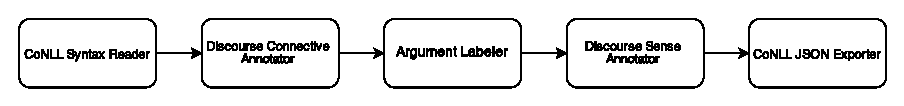
\includegraphics[width=18in]{CLaCDiscourseParser-crop.eps}
\end{center}
\end{textblock}

\begin{textblock}{4}(12,7.5)

Parses syntactic information provided by CoNLL and adds this information to the documents in the UIMA framework.
\end{textblock}

\begin{textblock}{4}(16.7,7.5)
Marks discourse usage or non-discourse usage of discourse connectives.
\end{textblock}

\begin{textblock}{4}(21.4,7.5)
Labels \textsc{Arg1} and \textsc{Arg2}.
\end{textblock}

\begin{textblock}{4}(26.1,7.5)
Disambiguates the sense of the discourse connective.
\end{textblock}

\begin{textblock}{4}(30.8,7.5)
Reads  the  output discourse  relations  annotated  in  the  UIMA  documents  and  generates  a  JSON  file.
\end{textblock}

\begin{textblock}{10}(36,4.5)
\CHead{III. Discourse Connective Annotator}
\textbf{Algorithm:}

\begin{itemize}
\item Searches the input texts for terms that match a predefined list of discourse connectives (was built solely from the CoNLL training dataset.

\item Checks each match of discourse connective to see if it occurs in discourse usage or not. 
\begin{itemize}
\item Uses a binary classifier with six features (i.e. F\textsubscript{1}-F\textsubscript{6})
\end{itemize}
\end{itemize}

\textbf{Results:}

\begin{itemize}
\item F\textsubscript{1} = 90.19\%.
\end{itemize}

\end{textblock}

\begin{textblock}{10}(00,10.5)
\CHead{IV. Argument Labeler}
\textbf{Algorithm}:
\begin{itemize}
\item Calculates the \textit{Connective-Root path nodes}, the nodes that appear in the path from the discourse connective to the root of the sentence.
\item Labels all constituents that are directly connected to one of the \textit{Connective-Root path nodes} with `part of \textsc{Arg1}', `part of \textsc{Arg2}' or `\textsc{Non}'.
\begin{itemize}
\item Uses a classifier with nine features (i.e. F\textsubscript{1}-F\textsubscript{9}).
\end{itemize}
\item Merges all constituents which were tagged as part of \textsc{Arg1} or as part of \textsc{Arg2} to obtain the actual boundaries of \textsc{Arg1} and \textsc{Arg2}.
\item If no constituent was labeled as a part of \textsc{Arg1}, the whole text of the previous sentence is considered as \textsc{Arg1}.
\end{itemize}

\textbf{Results}:
\begin{itemize}
\item The F\textsubscript{1} score of the \textit{Argument Labeler}:
\end{itemize}

\begin{table}[]
\centering
\begin{tabular}{|l|l|l|}
\hline
    & \textbf{Arg1}    & \textbf{Arg2}    \\ \hline
Best Result    & 49.68\% & 74.29\% \\
\textbf{CLaC Discourse Parser}    & \textbf{45.18\%} & \textbf{69.18\%} \\
Average & 30.77\% & 50.91\% \\ \hline
Std. deviation     & 15.31\% & 20.58\% \\ \hline
\end{tabular}
\label{tab:arg}
\end{table}
\begin{itemize}
\item Results show that the identification of \textsc{Arg1} is more difficult than \textsc{Arg2}.
\end{itemize}

\textbf{Error Analysis}:
\setstcolor{red}
\begin{itemize}
\item \textit{Attribute spans}:
\begin{itemize}
\item \st{But the RTC also requires ``working'' capital} \textit{to maintain the bad assets of thrifts that are sold} \underline{until} \textbf{the assets can be sold separately}.
\end{itemize}
\item Subordinate and coordinate clauses:
\begin{itemize}
\item \textit{We would have to wait} \underline{until} \textbf{we have collected on those assets} \st{before we can move forward.}
\end{itemize}
\end{itemize}

\end{textblock}



\begin{textblock}{10}(12,10.5)
\CHead{V. Features}

\begin{table}[!htb]
  \centering
  \begin{tabular}{|p{.3\textwidth}|p{.7\textwidth}|}
  \hline
  
    \textbf{Category} & \textbf{Description}\\
    \hline
    \hline
    \multirow{6}{*}{\parbox{.25\textwidth}{Connective Features}} 
    & F\textsubscript{1}: Discourse connective text in lowercase. \\ \cline{2-2}
    & F\textsubscript{2}: Categorization of the case of the connective: \textit{all lowercase}, \textit{all uppercase} and \textit{initial uppercase} \\ \cline{2-2}
    & F\textsubscript{3}: Highest node in the parse tree that covers the connective words but nothing more \\ \cline{2-2}
    & F\textsubscript{4}: Parent of \textit{SelfCat} \\ \cline{2-2}
    & F\textsubscript{5}: Left sibling of \textit{SelfCat} \\ \cline{2-2}
    & F\textsubscript{6}: Right sibling of \textit{SelfCat} \\ \hline
 
    \multirow{3}{*}{\parbox{.25\textwidth}{Syntactic Node Features}} 
    & F\textsubscript{7} Path from the node to the \textit{SelfCat} node in the parser tree \\ \cline{2-2}
    & F\textsubscript{8}: Context of the node in the parse tree. The context of a node is defined by its label the label of its parent, the label of left and right sibling in the parse tree. \\ \cline{2-2}
    & F\textsubscript{9}: Position of the node relative to the \textit{SelfCat} node: \textit{left} or \textit{right} \\ \hline
 
  \end{tabular}
\end{table}
\end{textblock}

\begin{textblock}{10}(24,10.5)
\CHead{VI. Example}

\textit{We would stop index arbitrage} \underline{when} \textbf{the market is under stress}.

\begin{center}
\resizebox{8in}{!}{
\Tree [ .S\textsubscript{1} [ .NP\textsubscript{1} [ .PRP We ] ] [ .VP\textsubscript{1} [ .MD would ] [ .VP\textsubscript{2} [ .VB stop ] \qroof{index arbitrage}.NP\textsubscript{2} [ .SBAR [ .WHADVP [ .WRB when ] ] \qroof{the market is under stress}.S\textsubscript{2} ] ] ] ] }
\end{center}

\begin{table}[]
\centering
\begin{tabular}{|l|l|}
\hline 
%F\textsubscript{1} = \emph{when} & F\textsubscript{4} = WHADVP & F\textsubscript{7} = $S \uparrow SBAR \downarrow WHADVP$ \\ \hline
%F\textsubscript{2} = all lowercase & F\textsubscript{5} = null & F\textsubscript{8} = S-SBAR-WHADVP-null \\ \hline
%F\textsubscript{3} = WRB & F\textsubscript{6} = S & F\textsubscript{9} = left \\ \hline

F\textsubscript{1} = \emph{when} & F\textsubscript{2} = all lowercase \\ \hline F\textsubscript{3} = WRB & F\textsubscript{4} = WHADVP \\ \hline
F\textsubscript{5} = null & F\textsubscript{6} = S \\ \hline
F\textsubscript{7} = $S \uparrow SBAR \downarrow WHADVP$  & F\textsubscript{8} = S-SBAR-WHADVP-null \\ \hline
F\textsubscript{9} = left &  \\  \hline
\end{tabular}
\end{table}

\end{textblock}


\begin{textblock}{10}(36,10.5)
\CHead{VII. Discourse Sense Annotator}
\begin{itemize}
\item Uses the na\"\i ve approach that labels each discourse connective with its most frequent. The most frequent relation for discourse connectives is mined from the CoNLL training dataset.
\end{itemize}
\end{textblock}


\begin{textblock}{22}(12,20.5)
\CHead{VIII. Overall Results}

\begin{itemize}
\item The F\textsubscript{1} scores of the CLaC discourse parser and the individual performance of its components:
\end{itemize}

\begin{table}[!htb]
\centering
\begin{tabular}{|l|r|r|r|r|}
\hline
                      & \parbox{.2\textwidth}{\textbf{Discourse Connective \\ Classifier}} & \parbox{.11\textwidth}{\textbf{Argument \\ Labeler}} & \parbox{.2\textwidth}{\textbf{Discourse Parsing \\ (explicit only)}} & \parbox{.2\textwidth}{\textbf{Discourse Parsing \\ (explicit and implicit)}} \\ \hline
Best Result           & 91.86\%      & 41.35\%          & 30.58\%         & 24.00\%  \\
\textbf{CLaC Discourse Parser}           & \textbf{90.19\%}          & \textbf{36.60\%}          & \textbf{27.32\%}        & \textbf{17.38\%} \\
Average               & 74.20\%          & 23.89\%          & 18.28\%        & 13.25\% \\ \hline
Standard deviation    & 23.24\%          & 13.01\%          & 9.93\%         & 6.41\% 
\\ \hline
\end{tabular}
\end{table}
\end{textblock}

\begin{textblock}{10}(36,13.5)
\CHead{IX. Conclusion}
\begin{itemize}
\item CLaC Discourse Parser was developed from scratch for CoNLL 2015. 
\item 3 person-month effort focused on \textit{Discourse Connective Classification} and \textit{Argument Labeler}. 
\item Na\"\i ve approach for sense labelling and consider only explicit relations. 
\item Yet, good results.
%\item The parser achieves an overall F\textsubscript{1} measure of 17.38\%, ranking in 6\textsuperscript{th} place out of the 17 parsers submitted to the CoNLL 2015 shared task.
\end{itemize}
\end{textblock}



\begin{textblock}{10}(36,17.5)
\bibliographystyle{plainnat}
\bibliography{discourse,resources}
\end{textblock}



\begin{textblock}{46}(00,25.5)
\begin{center}
{\footnotesize Contact information:
Email: \textsuperscript{$\ast$}\textit{m\_laali@encs.concordia.ca} \textsuperscript{$\dagger$}\textit{e\_davoo@encs.concordia.ca} \textsuperscript{$\ddagger$}\textit{kosseim@encs.concordia.ca}; 
Web: \textit{https://clac.encs.concordia.ca}
}
\vspace{-0.75\baselineskip}

%{\footnotesize Acknowledgments: The authors would like to thank the CoNLL 2015 organizers and the anonymous reviewers. This work was financially supported by NSERC.}
\end{center}
\end{textblock}

\end{document}
